\section{Motion Planning}
\label{sec:plan}
% Path planning, RRT*, anytime dynamic...
Motion planning in a dynamic environment requires agility and computational speed, such that the robot is able to check the status of the environment in cycles that allow sufficient anticipation to obstacle that are moving. A previous offline plan can be made before the operation starts, but then, the robot needs to update it with information from sensors, being able to change or replan when other bodies obstruct the trajectory.

\subsection{RRT*}
\label{sec:rrt}
The RRT* algorithm, also called RRT-connect, is an improved extension of the original RRT (Rapidly-exploring Random Tree). This algorithm is used to search for collision-free paths in high dimensional spaces, such as the Configuration Space (C-space) of the robot. Initially, it is given the \textit{map} of the C-space itself, an initial configuration \textit{Q\_start} and a final goal configuration \textit{Q\_goal}. It works by constructing a space-filling tree of nodes based on random exploration of the space, extending nodes by a fixed distance (epsilon parameter). Each node represents an intermediate \textit{Q} vector to move from start to goal. \\

The original RRT was designed to start the tree and grow only in one direction, from the starting node to the goal. RRT*, however, uses both input configurations (\textit{Q\_start} and \textit{Q\_goal)}, starting a tree in both and growing with the attempt to match both trees, which solves the path in shorter time. Figures \ref{fig:rrt} and \ref{fig:rrs} illustrate both RRT and RRT* algorithms.\\

\begin{figure}[ht!]
\centering
\begin{minipage}{.5\textwidth}
  \centering
  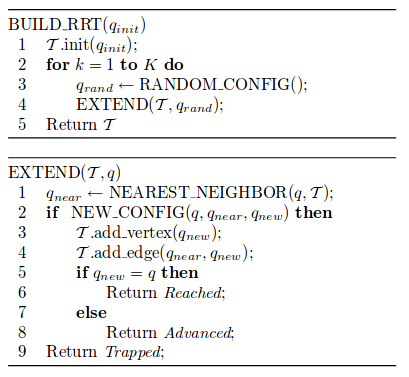
\includegraphics[width=1\linewidth]{Images/plan/RRT.png}
  \captionof{figure}{RRT algorithm. Source: \cite{RRTConnect}.}
  \label{fig:rrt}
\end{minipage}%
\begin{minipage}{.5\textwidth}
  \centering
  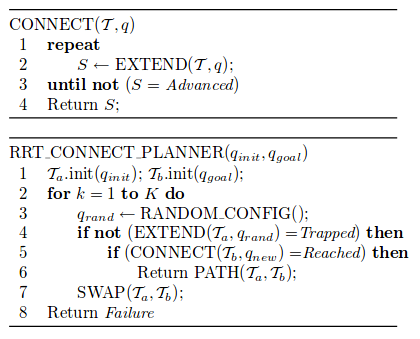
\includegraphics[width=1\linewidth]{Images/plan/RRTstar.png}
  \captionof{figure}{RRT* algorithm. Source: \cite{RRTConnect}.}
  \label{fig:rrs}
\end{minipage}
\end{figure}

The size and the run-time of the RRT* depends a lot in the size of the epsilon (extend) parameter. In operations in which the robot motion can be solved offline, and therefore there is plenty of time for the algorithm to work, RRT* tends to find optimal path solutions. However, our task is time-demanding, and therefore the path calculation time has to be kept to a minimum. The tree methodology of RRT* is very suitable for obstacle avoidance since it is able to produce solutions at anytime, but these solutions are not optimal and therefore, path optimization methods have to be used to improve the efficiency of the system.


\subsection{Online Planning}
\label{sec:onl}

The RRT* itself is not self-reconfigurating. It has no implementation of a functionality to periodically receive new environment information and update the C-space in search of possible collisions, nor the ability of replanning. To solve this problem Dynamic RRT* is used. With this improvement, it is possible to replan efficiently (without doing it from scratch) based on obstacle detection by the system's sensor. The online planner is constructed as follows:\\

\begin{algorithm}
\caption{Online Planner Dynamic RRT*}\label{planner}
\begin{algorithmic}[1]
\Procedure{Procedure}{}
\State \emph{loop}:
    \State $\textit{Initialize(Tree, q\_start, q\_goal)}$
    \State $\text{path} \gets \textit{planRRT*(Tree)}$
    \State $\textit{postSolution(path)}$
    \State $\text{obstacles} \gets \textit{findObstacles()}$
    \ForAll{$\textit{obstacles}$}
        \State  $\textit{InvalidateNodes(Tree, obstacles)}$
    \EndFor
        \If {$\textit{path} \text{ contains invalidated nodes}$}
            \State $\text{path} \gets \textit{replanRRT(Tree)}$
            \State $\textit{postSolution(path)}$
        \EndIf 
    \State $\textit{updateParameters(Tree)}$
\EndProcedure
\end{algorithmic}
\end{algorithm}

The planner starts the tree and calculates an initial path with the starting state of the workspace. As the robot starts moving, it keeps receiving data from the camera about the location of the moving obstacles. This data is processed online, and the system checks for collisions inside the path. This is done by filtering the nodes of the path in a collision detector that contrasts the position of the arm in each node with the current location of the ball (derived from the latest coordinates received from the camera). If any of this nodes is in collision, planner invalidates it, and cuts the tree at that point. Then, it replans from there a new path to the goal that avoids the obstacle. In the mean time, the collision detector keeps running and this process is repeated again if a new collision is found due to new updated locations of the obstacle.  \\

When the system does not detect collisions, and there exist already a calculated collision free path, the robot just keeps moving to the goal until the collision detector tells the contrary. This combination of RRT* and dynamic planning allows for fast replanning when necessary, otherwise fast collision free path planning for the robot to get to the goal \cite{connell}. \\

\subsection{Path Optimization}
\label{sec:opt}

As we stated previously, at fast computation times, the solutions provided by the planner are far from being optimal. Usually, these solutions contain a lot of unnecessary and/or redundant nodes along the path. In order to improve this inefficient paths, we used the optimization method called path pruning. This operation eliminates all nodes $n_{i}$ whose prior $n_{i-1}$ and posterior nodes $n_{i+1}$ are both collision free. It is a deterministic technique, meaning that it always return the same solution for the same given input state. The algorithm is shown in figure \ref{fig:prun}. \\

\begin{figure}[ht!]
    \centering
    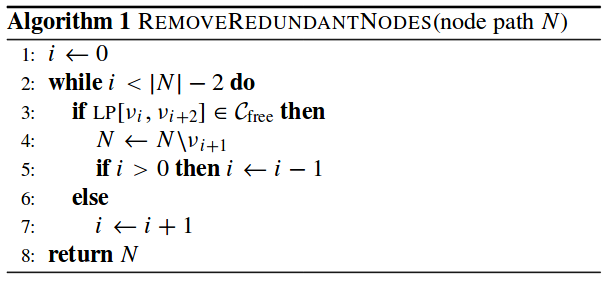
\includegraphics[width=0.7\textwidth]{Images/plan/pruning.png}
    \caption{Path pruning algorithm. Source: \cite{optimization}}
    \label{fig:prun}
\end{figure}

We chose this optimization solution over others available for several reasons. Firstly, since RRT* produces paths that are composed by a discrete sequence of nodes, pruning is a perfectly suitable complement to it. Secondly, obstacle avoidance requires computational speed, and pruning is a fast method. The main drawback of this method is that it may reduce the clearance between the obstacle and the robot. However, for that reason, the obstacle model has been already built with sufficient clearance in the radius size, to prevent from this situation. \\